\documentclass[11pt]{scrartcl}
%%
%
% This is a poster template with latex macros and using
% the University of Florida Logo.  For further information
% on making postscript, resizeing, and printing the poster file
% please see web site 
% http://www.phys.ufl.edu/~pjh/posters/poster_howto.html
% 
% N.B. This format is cribbed from one obtained from the University
% of Karlsruhe, so some macro names and parameters are in German
% Here is a short glosary:
% Breite: width
% Hoehe: height
% Spalte: column
% Kasten: box
%
% All style files necessary are part of standard TeTeX distribution
% On the UF unix cluster you should not need to import these files
% specially, as they will be automatically located.  If you
% run on a local PC however, you will need to locate these files.
% At UF try /usr/local/TeTeX...
% 
% P. Hirschfeld 2/11/00
%
% The recommended procedure is to first generate a ``Special Format" size poster
% file, which is relatively easy to manipulate and view.  It can be
% resized later to A0 (900 x 1100 mm) full poster size, or A4 or Letter size
% as desired (see web site).  Note the large format printers currently
% in use at UF's OIR have max width of about 90cm or 3 ft., but the paper
% comes in rolls so the length is variable.  See below the specifications
% for width and height of various formats.  Default in the template is
% ``Special Format",  with 4 columns.
%%
%% 
%% Choose your poster size:
%% For printing you will later RESIZE your poster by a factor
%%        2*sqrt(2) = 2.828    (for A0)
%%        2         = 2.00     (for A1) 
%%  
%% 
\def\breite{350mm}     % Special Format. 
\def\hoehe{494mm}      % Scaled by 2.82 this gives 110cm x 90cm 

%\def\breite{390mm}     % Special Format. 
%\def\hoehe{319.2mm}      % Scaled by 2.82 this gives 110cm x 90cm 
\def\anzspalten{2}
%%
%%\def\breite{420mm}     % A3 LANDSCAPE
%%\def\hoehe{297mm}
%%\def\anzspalten{4}
%%
%% \def\breite{297mm}     % A3 PORTRAIT
%% \def\hoehe{420mm}
%% \def\anzspalten{3}
%%
%% \def\breite{210mm}     % A4 PORTRAIT
%% \def\hoehe{297mm}
%% \def\anzspalten{2}
%%
%%
%% Procedure:
%%   Generate poster.dvi with latex
%%   Check with Ghostview
%%   Make a .ps-file with ``dvips -o poster.ps poster''
%%   Scale it with poster_resize poster.ps S
%%   where S is scale factor
%%     for Special Format->A0 S= 2.828 (= 2^(3/2)))
%%     for Special Format->A1 S= 2 (= 2^(2/2)))
%% 
%% Sizes (European:)
%%   A3: 29.73 X 42.04 cm
%%   A1: 59.5 X 84.1 cm
%%   A0: 84.1 X 118.9 cm
%%   N.B. The recommended procedure is ``Special Format x 2.82"
%%   which gives 90cm x 110cm (not quite A0 dimensions).
%%
%% --------------------------------------------------------------------------
%%
%% Load the necessary packages
%% 
\usepackage{palatino}
\usepackage[utf8]{inputenc}
\usepackage{epsf}
\usepackage{graphicx,psfrag,color,pstcol,pst-grad}
\usepackage{amsmath,amssymb}
\usepackage{latexsym}
\usepackage{calc}
\usepackage{multicol}
%%
%% Define the required numbers, lengths and boxes 
%%
\newsavebox{\dummybox}
\newsavebox{\spalten}
%\input psfig.sty

%%
%%
\newlength{\bgwidth}\newlength{\bgheight}
\setlength\bgheight{\hoehe} \addtolength\bgheight{-1mm}
\setlength\bgwidth{\breite} \addtolength\bgwidth{-1mm}

\newlength{\kastenwidth}

%% Set paper format
\setlength\paperheight{\hoehe}                                             
\setlength\paperwidth{\breite}
\special{papersize=\breite,\hoehe}

\topmargin -1in
\marginparsep0mm
\marginparwidth0mm
\headheight0mm
\headsep0mm


%% Minimal Margins to Make Correct Bounding Box
%\setlength{\oddsidemargin}{-2.44cm}
%\addtolength{\topmargin}{-3mm}
\setlength{\oddsidemargin}{-2.44cm}
\addtolength{\topmargin}{-3mm}
\textwidth\paperwidth
\textheight\paperheight

%%
%%
\parindent0cm
\parskip1.5ex plus0.5ex minus 0.5ex
\pagestyle{empty}




\definecolor{recoilcolor}{rgb}{1,0,0}
\definecolor{occolor}{rgb}{0,1,0}
\definecolor{pink}{rgb}{0,1,1}





\def\UberStil{\normalfont\sffamily\bfseries\large}
\def\UnterStil{\normalfont\sffamily\small}
\def\LabelStil{\normalfont\sffamily\tiny}
\def\LegStil{\normalfont\sffamily\tiny}

%%
%% Define some commands
%%
\definecolor{JG}{rgb}{0.1,0.9,0.3}

\newenvironment{kasten}{
  \begin{lrbox}{\dummybox}
    \begin{minipage}{\linewidth}}
    {\end{minipage}
  \end{lrbox}
  \raisebox{-\depth}{\psshadowbox[cornersize=absolute,linearc=14pt,framesep=1em]{\usebox{\dummybox}}}\\[0.5em]}
\newenvironment{spalte}{
  \setlength\kastenwidth{1.2\textwidth}
  \divide\kastenwidth by \anzspalten
  \begin{minipage}[t]{\kastenwidth}}{\end{minipage}}

%\renewcommand{\emph}[1]{{\color{red}\textbf{#1}}}


%\def\op#1{\hat{#1}}
\begin{document}
%%%%%%%%%%%%%%%%%%%%%%%%%%%%%%%%%%%%%%%%%%%%%%%%%%%%
%%%               Background                     %%%
%%%%%%%%%%%%%%%%%%%%%%%%%%%%%%%%%%%%%%%%%%%%%%%%%%%%
{\newrgbcolor{gradbegin}{0.5 0.5 1}
  \newrgbcolor{gradend}{1 1 1}%{1 1 0.5}%
  %\rput[cm](15.23,-15){
  \rput[tl]{0}(0,0){
  %\includegraphics[width=\paperwidth]{images/background}
  }
\vfill}

%{\newrgbcolor{gradbegin}{0.5 0.5 1}%
%  \newrgbcolor{gradend}{1 1 1}%{1 1 0.5}%
%  \psframe[fillstyle=gradient,gradend=gradend,%
%  gradbegin=gradbegin,gradmidpoint=0.1](\bgwidth,-\bgheight)}
%\vfill
%%%%%%%%%%%%%%%%%%%%%%%%%%%%%%%%%%%%%%%%%%%%%%%%%%%%
%%%                     Header                   %%%
%%%%%%%%%%%%%%%%%%%%%%%%%%%%%%%%%%%%%%%%%%%%%%%%%%%%
\hfill
\psshadowbox{\makebox[0.95\textwidth]{%
    \hfill
	\parbox[c]{2cm}{\includegraphics[width=2cm,height=!]{images/alma_logo}}
    \hfill
    \parbox[c]{0.7\linewidth}{%
      \begin{center}
		\textbf{\Huge {A Reference Architecture Specification of a\\
		Generic Telescope Control System}}\\[0.5em]
		\textsc{\large Joao S. L\'opez$^{1}$, Rodrigo J. Tobar$^{1}$,
		Tomas Staig$^{1}$, Daniel A. Bustamante$^{1}$,\\ Camilo E.
		Menay$^{1}$, Mauricio A. Araya$^{2}$ and Horst H. von
		Brand$^{1}$}\\[0.3em] { $^1$Computer Systems Research Group,
		Universidad T\'ecnica Federico Santa Mar\'ia (UTFSM),
		Valpara\'iso, Chile}\\ { $^2$Institut National de Recherche en
		Informatique et Automatique (INRIA), Nancy, France}
      \end{center}}
	\hfill
    \parbox[c]{2cm}{\includegraphics[width=3cm,height=!]{images/utfsm_logo}}
	\hfill
\hfill}}\hfill\mbox{}\\

\hfill
\psshadowbox{\makebox[0.83\textwidth]{%
    \hfill
    \parbox[t]{0.8\linewidth}{%
\hfill{\large\bf{\color{red}ABSTRACT}}\hfill\mbox{}\\
A Telescope Control System (TCS) is a software responsible of controlling the
hardware that an astronomical observation needs. The automation and
sophistication of these observations has produced complex systems. Currently, a
TCS is compound by software components that interact with several users and even
with other systems and instruments.\\

Each observatory has successfully developed a wide spectrum of TCS solutions to
their telescopes. Regardless the mount, there are common patterns in the
software components that all these telescopes use. As almost every telescope is
custom designed, these patterns are reimplemented again and again for each
telescope. This is indeed an opportunity of reuse and collaboration.\\

The Generic Telescope Control System (gTCS) pretends to be a base distributed
framework for the developing and deployment of the TCS of any telescope,
independent of its physical structure, the type of mount and instrumentation
that they use. This work presents an architecture specification explained
through two complementary approaches: the layers perspective and the deployment
perspective. The first approach defines a set of layers, one on the top of the
other, offering different levels of abstraction. Meanwhile the deployment
perspective intends to illustrate how the system could be deployed, focused on
the distributed nature of the devices.\\
}
\hfill}}\hfill\mbox{}

\begin{lrbox}{\spalten}
  \parbox[t][0.61\textheight]{1.3\textwidth}{
   % \vspace*{0.2cm}
%%%%%%%%%%%%%%%%%%%%%%%%%%%%%%%%%%%%%%%%%%%%%%%%%%%%
%%%                 first column                 %%%             
%%%%%%%%%%%%%%%%%%%%%%%%%%%%%%%%%%%%%%%%%%%%%%%%%%%%
    \begin{spalte}
     
      \begin{kasten}
		\section*{\hspace{0.1cm} {\color{red} The Generic TCS Problem}}
        \subsection*{\hspace{0.2cm} {\color{blue} Overview}}
			\begin{minipage}[t]{0.95\linewidth}
Control systems have two basic entry points: the \textit{users} and the
\textit{devices}. In a TCS domain, users and devices are heterogeneous: users
with various levels of expertise, and devices with different protocols and
access levels. Therefore, to understand the problem we must identify the diverse
nature of users and devices. \\
			\end{minipage}

        \subsection*{\hspace{0.2cm} {\color{blue} The Users}}

			\begin{minipage}[t]{0.45\linewidth}
Users can be classified by the \emph{usage} that they give to the system, or in
other words, to which \emph{profile} they belong. Profile examples:

\begin{itemize}
	\item \textbf{Observation Control}: The control of the observation
itself. Includes all the variables in the domain of the Astronomer, and all the
technical and specific details of the telescopes are hidden.
	\item \textbf{Calibration and Startup}: The automatic or manual process
of calibrating the telescope, also in high-level domain, but including the
specific details of the telescope.
	\item \textbf{Maintenance}: The low-level variables of the telescope,
with a detailed control of all the devices and software states.
	\item \textbf{Monitoring}: The summary of the telescope operations to
audit, check the behavior of the devices, etc. This may be a mixture of specific
logs with general information of the observation.
\end{itemize}

			\end{minipage}
			\begin{minipage}[t]{0.5\linewidth}
			\strut\vskip -\baselineskip
			\hspace{0.8cm}
			\includegraphics[width=1\linewidth,height=!]{images/users}
			\end{minipage} \hfill

			\begin{minipage}[t]{0.95\linewidth}
\vspace{0.5cm}
The problem is that several users could use more than one profile. Then,
building an application for each profile is not the most desired approach.
Therefore, the existing TCSs often builds very complex user interfaces that have
all the possible variables that the user \emph{may} need. This turns the
application unmanageable for unexperienced users. Fortunately, defining these
profiles helps to identify which is the scope of the TCS and select the features
that the system will need in a user-independent fashion.\\
			\end{minipage}

        \subsection*{\hspace{0.2cm} {\color{blue} Devices Scope}}

			\begin{minipage}[t]{0.95\linewidth}
The devices of a telescope are diverse. Only in the axis control domain each
telescope mount/technology has different devices with different protocols and
configurations. Even if two telescopes has the same hardware, the firmware or
other vendor software could vary. If we add to the equation mirror control,
active optics and meteorologic stations, the set of devices turns unmanageable.
Therefore, defining the possible set of devices is not a practical approach. A
simpler approach is to group the devices into \emph{instruments} that do a
specific task.  In an observatory there are two general types of hardware
devices:

\begin{itemize}
	\item \textbf{Technical Instruments}: All instrument that does not
directly produce scientific data, such as the telescope, a meteorologic station,
the active optics, an autoguiding CCD, etc.
	\item \textbf{Scientific Instruments}: All instrument that produces
scientific data that the astronomer will use, such as the main CCD, a
spectrograph, an interferometer, filter wheels, etc.  \end{itemize}

The scope of a TCS is limited to \emph{technical instruments} and their devices.
Also, a TCS must provide all the interfaces to connect the software in charge of
managing the \emph{scientific instruments}. \\

			\end{minipage}
      \end{kasten}

    \end{spalte}
	 \hfill
%%%%%%%%%%%%%%%%%%%%%%%%%%%%%%%%%%%%%%%%%%%%%%%%%%%%
%%%               second column                  %%%             
%%%%%%%%%%%%%%%%%%%%%%%%%%%%%%%%%%%%%%%%%%%%%%%%%%%%
    \begin{spalte}
       
      \begin{kasten}
        \section*{\hspace{0.1cm} {\color{red} Proposed Architecture
	Specification}}
        \subsection*{\hspace{0.2cm} {\color{blue} Layers perspective}}
			\begin{minipage}[t]{0.45\linewidth}
The \emph{layers perspective} presents different levels of abstraction (higher
layers offer higher abstractions). This perspective can be seen as the network
stack (such TCP/IP) where each layer offers services to the upper one, and the
upper one only uses the lower one. 

This view allow us to have an idea of which are the different abstractions
that the system needs, and how to encapsulate this information in different
layers.

\begin{description}
	\item[Drivers] Responsible of the communication of the system with
		external entities.
	\item[Sensors/Actuators] It provides software abstractions of physical
		devices, without considering any interaction with any other
		device.
	\item[Composite devices] It represents a full device used on the
		astronomy domain, and that can be composed by a given number of
		sensors and/or actuators.
\end{description}

			\end{minipage}
			\begin{minipage}[t]{0.5\linewidth}
			\strut\vskip -\baselineskip
			\hspace{0.8cm}
			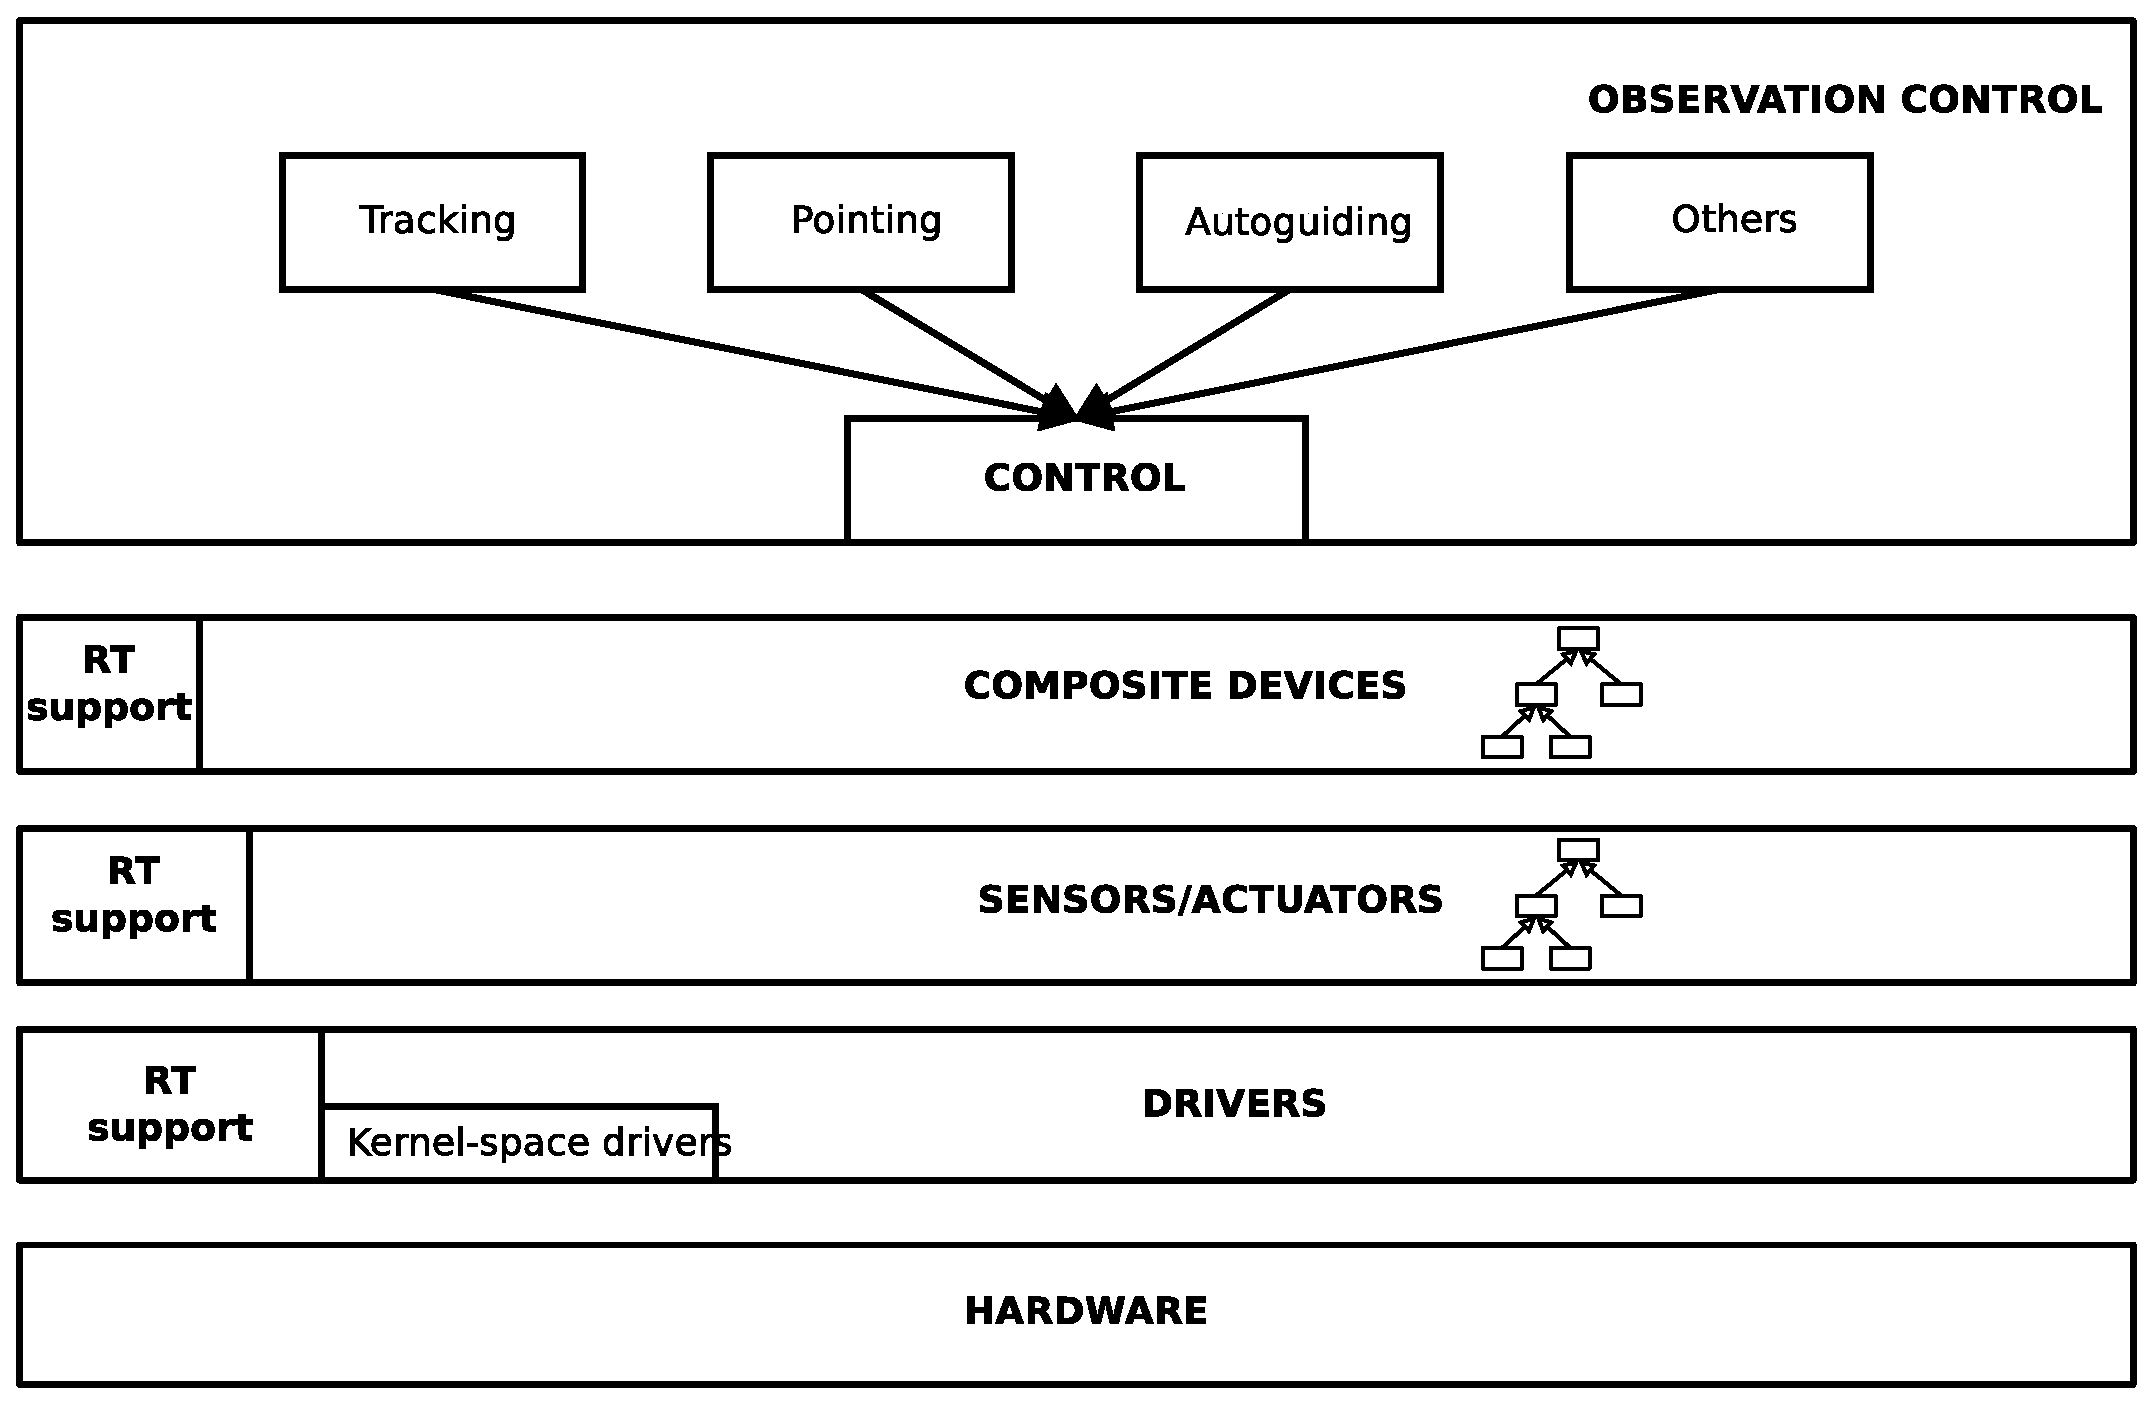
\includegraphics[width=1\linewidth,height=!]{images/layers}
			\end{minipage} \hfill

			\begin{minipage}[t]{0.95\linewidth}
\vspace{0.3cm}
\begin{description}
	\item[Observation control] It offers the abstraction of a full equipped
		and controlled telescope. This is done by grouping different
		composite devices, and using them in a intelligent way, in order
		to obtain data, collaborate, and finally do control over the
		necessary composite devices.
\end{description}

			\end{minipage}

        \subsection*{\hspace{0.2cm} {\color{blue} Deployment perspective}}
			\begin{minipage}[t]{0.45\linewidth}
The \emph{deployment perspective} intends to illustrate how the architecture can
be used in a distributed way. It shows the geographical distribution of the
system, and the bus that communicates the different parts of the system.

Each computer will execute different parts of the system. We can distribute one
layer through different computers. This is the capability of the system to have
its components distributed over a network of computers, but working together. 

The Information Service can be seen as a software component accessible through
any part part of the system. It has two main responsibilities: to know which
software components are available in the system and to offer the possibility to
retrieve information about the classes, interfaces, methods, parameters and
related information from all the components of the system.\\

			\end{minipage}
			\begin{minipage}[t]{0.5\linewidth}
			\strut\vskip -\baselineskip
			\hspace{0.8cm}
			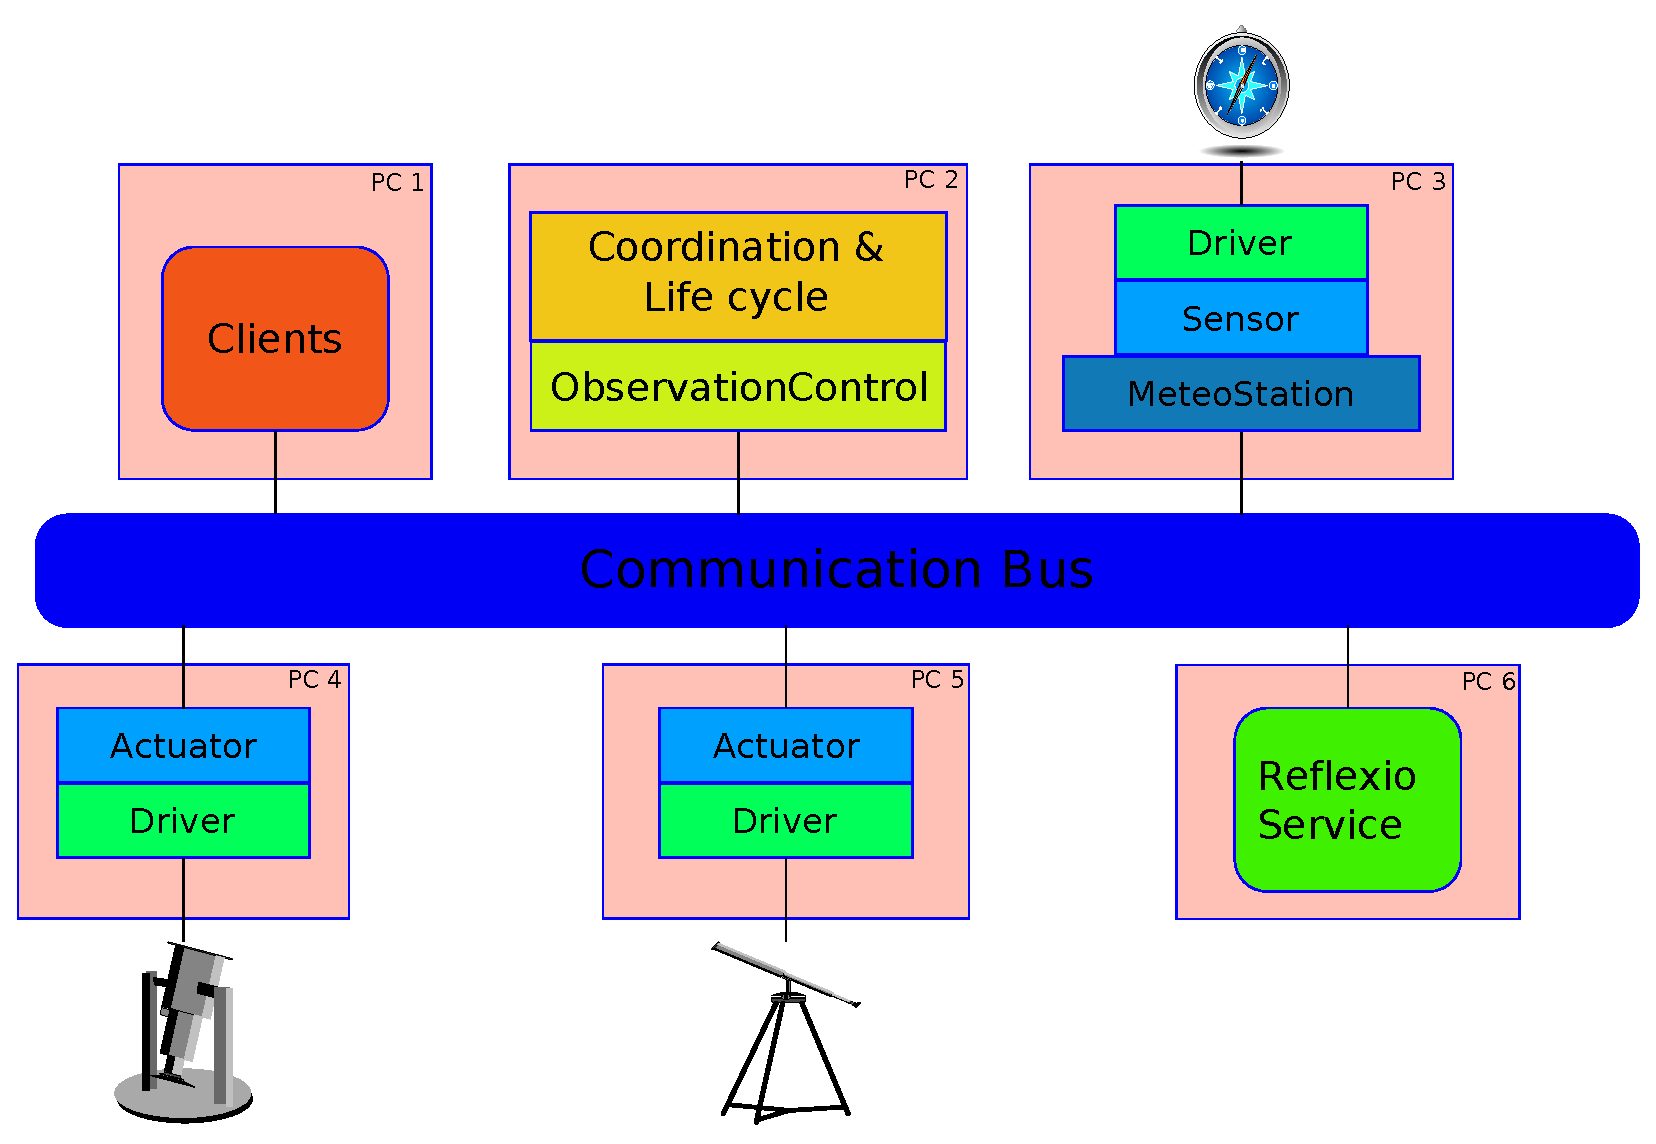
\includegraphics[width=1\linewidth,height=!]{images/deploy-view}
			\end{minipage} \hfill

      \end{kasten}

    \end{spalte}
	 \hfill\mbox{}

}
\end{lrbox}
\hfill
\resizebox*{0.95\textwidth}{!}{
  \usebox{\spalten}}\hfill\mbox{}

\vspace{-2cm}
\hspace{1cm}
\psshadowbox[cornersize=absolute,linearc=14pt]{\makebox[0.923\textwidth]{%
	 \hfill
    \parbox[t]{0.9\linewidth}{
\begin{minipage}[t]{0.49\linewidth}
\vspace{0.1cm}
\section*{ {\normalsize \color{red} Reference technologies}}

{\footnotesize
\renewcommand{\baselinestretch}{0.5}
The Control System for an Amateur Telescope~[1] project, a TCS constructed over
ALMA Common Software (ACS)~[2,3] was used as an initial approach to the problem and
reference architecture.

To exemplify the proposed reference, existing technologies that are implementing
some aspects of the proposal are analyzed.

\begin{description}
	\item[ALMA Common Software] If we consider the Container/Component~[4]
		model present on ACS, each composite device can be managed by an
		ACS Characteristic component. Through the use of states,
		exceptions and container lifecycle we are able to manage the
		lifecycle of the whole gTCS. Currently ACS uses CORBA, which is
		an example of a communication bus. The information service can
		be obtained through the Manager (responsible for the management
		of containers, components and clients) and the information
		provided by the Interface Repository (IR) and the Configuration
		Database (CDB).
\end{description}

}
\end{minipage}\hfill
\begin{minipage}[t]{0.49\linewidth}
\vspace{0.8cm}
{\footnotesize
\renewcommand{\baselinestretch}{0.5}

\begin{description}
	\item[VLT Common Software] The VLT control software~[5] uses software
		modules, sharing benefits of re-usability. These modules are a
		basic item for the detailed design, development and integration
		of software.  The software architecture is distributed over
		several workstations that provide high level and coordination
		services. The communication is based on a message system and a
		distributed hierarchical database.
		
	\item[Java Remote Method Invocation] The Java Remote Method Invocation
		(RMI)~[6] is a Java approach to support a model of a distributed
		object application. It provides remote communication between
		programs written in Java. It allows applications to call
		methods located remotely, sharing resources and processing load
		across systems.
\end{description}
}
\end{minipage}
}
\hfill}}\hfill\mbox{}\\
\vfill

\hfill
\psshadowbox{\makebox[0.922\linewidth]{
\hfill
\begin{minipage}[t]{0.25\linewidth}
{\scriptsize
{\small\bf Acknowledgements}

\renewcommand{\baselinestretch}{0.5}

This work was supported by ALMA-CONICYT Fund project \#31060008 \textit{``Software
Development for ALMA: Building Up Expertise to Meet ALMA Software Requirements
withing a Chilean University''}, under development at Universidad T\'ecnica
Federico Santa Mar\'ia.
}
\end{minipage} \hfill

\begin{minipage}[t]{0.65\linewidth}
{\scriptsize
\renewcommand{\baselinestretch}{1.0}
{\small\bf References}

[1] Tobar, R. et~al., ``An amateur telescope control system towards a generic
telescope control model'' in [{\em Proceedings of SPIE - Advanced Software and
Control for Astronomy 2008}{\hspace{0.1em}}], (2008).
\renewcommand{\baselinestretch}{0.5}

[2] Chiozzi, G. et~al., ``The ALMA Common Software: A developer friendly CORBA
based framework'' in [{\em Proceedings of SPIE - Advanced Software and Control
for Astronomy 2004}{\hspace{0.1em}}], (2008).
\renewcommand{\baselinestretch}{0.5}

[3] Chiozzi, G. et~al., ``Application development using the ALMA Common
Software'' in [{\em Proceedings of SPIE - Advanced Software and Control for
Astronomy 2006}{\hspace{0.1em}}], (2006).  
\renewcommand{\baselinestretch}{0.5}

[4] Sommer, H. et~al., ``Container-component model and XML in ALMA ACS'' in
[{\em Proceedings of SPIE - Advanced Software and Control for Astronomy
2004}{\hspace{0.1em}}], (2004).
\renewcommand{\baselinestretch}{0.5}

[5] Chiozzi, G., ``An object-oriented event-driven architecture for the VLT Telescope Control Software'' in
[{\em Proceedings of ICALEPCS 1995
}{\hspace{0.1em}}], (1995).
\renewcommand{\baselinestretch}{0.5}

[6] Grosso, W., ``Java RMI'', O'Reilly \& Associates Inc, (2002).
\renewcommand{\baselinestretch}{0.5}

}
\hfill
\end{minipage}
}}\hfill\mbox{}




\hfill
\psshadowbox{\makebox[0.95\linewidth]{
\begin{minipage}[t]{0.15\linewidth}
	\begin{tabular}{ccc}
	
\includegraphics[width=!,height=1.5cm]{images/eso_logo} &
	
\includegraphics[width=!,height=1.5cm]{images/nrao_logo} &
	
\includegraphics[width=!,height=1.5cm]{images/naoj_logo}
	\end{tabular}
\end{minipage} \hfill
\begin{minipage}[t]{0.50\linewidth}
	\begin{center}
	\Huge{Atacama Large Millimeter Array}
	\end{center}
\end{minipage} \hfill
\begin{minipage}[t]{0.10\linewidth}
	%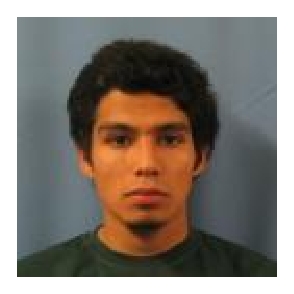
\includegraphics[width=!,height=1.5cm]{logos/authorpic}
\end{minipage}
}}\hfill\mbox{}


\vfill
\hfill
{\scriptsize
Contact e-mail: {\color{blue}jslopez@csrg.inf.utfsm.cl} /
For more information about ALMA developement and research at UTFSM Computer
Systems Research Group, please visit our web site {\color{blue}http://alma.inf.utfsm.cl}
}
\hfill
\ 

\end{document}
